\section{Segmentation of the MILP problem}
\label{section:segment}
\subsection{Introduction}
The model described in the previous section is enough to find a path, but the solver will take a very long time when the length of the path and the amount of obstacles are increased. This section presents the preprocessing pipeline that makes the problem more scalable. The first step is finding an initial path with the Theta* algorithm. The second step is finding the corners in that path. The third step is generating segments based on those corners. Finally, the obstacles to be modeled in the MILP problem are selected while the others are approximated with a genetic algorithm. The goal is to segment the problem in such a way that only a minimal amount of obstacles need to be modeled in each segment, while still resulting in a relatively fast path. As the segments get smaller, fewer obstacles need to be modeled. However, the path will also become slower. By increasing the size of the segment, the path will get closer to the optimal path, but at a performance penalty because much more obstacles need to be modeled.\\
For the best results, we want to find segments which are as large as possible but contain as few obstacles as possible. By generating a segment for each corner in the path, we can make the segments just large enough so the vehicle can always slow down in time to navigate the corner. This way the vehicle will always navigate corners  efficiently, without making the segments too large to solve in an acceptable amount of time.
\subsection{Finding the initial path}
\begin{figure*}[!t]
    \centering
    \subfloat{
        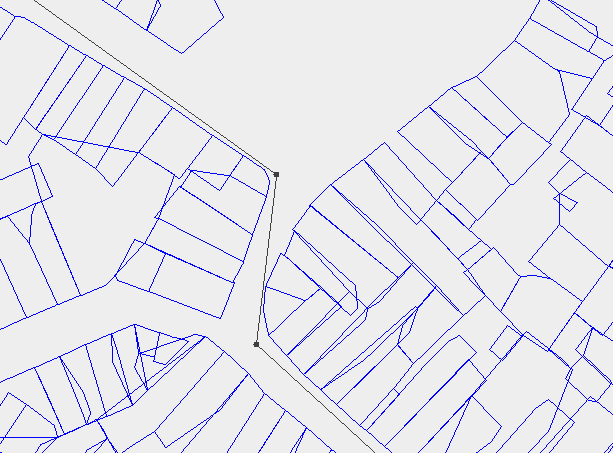
\includegraphics[width=0.48\textwidth]{img/pre1}
    }
    \hfil
     \subfloat{
        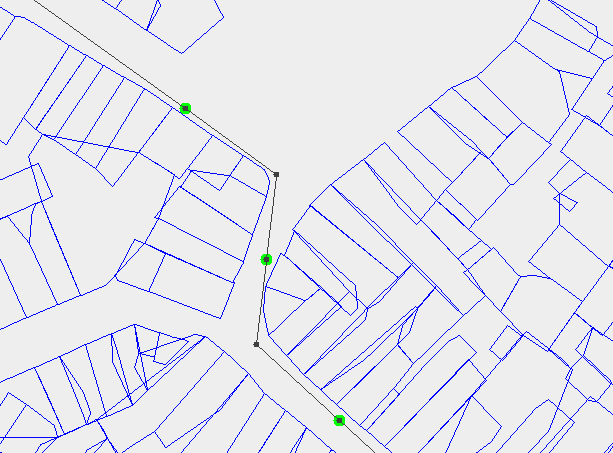
\includegraphics[width=0.48\textwidth]{img/pre2}
     }
    \caption{The left image shows the results after the Theta* algorithm has executed. The blue shapes are obstacles, while the gray line is the Theta* path. The right image shows the results after the path is segmented. Extra nodes have been added to the Theta* path, as marked by the green circles. These circles depict the transitions between segments.}\label{fig:pre-1-2}
\end{figure*}
The first issue is that because the goal cannot be reached immediately, the goal function for the MILP problem needs to change.  \\
One option is to simply get as close as possible to the goal during each segment. Because the distance that can be traveled during a segment is limited, the amount of obstacles that need to be modeled is also limited. This works well when the world is very open with little obstacles. However, this greedy approach is prone to getting stuck in dead ends in more dense worlds like cities.
\\
The second option is finding a complete path using a method that's easier to compute. An algorithm like A* can be used to find a rough estimation for the path. This A* path is the shortest path, but does not take constraints or the characteristics of the vehicle into account. A very curvy direct path may be the shortest, but a detour which is mostly straight and allows for higher speeds may actually be faster. 
\\
It is possible to use more advanced algorithms that model more of the constraints. This will significantly improve the execution time of the MILP solver and quality of the solution, but it will also come at a performance cost. A balance needs to be found between the execution time of the preprocessing step and that of the MILP solver. The preprocessing step needs to do just enough so the solver can find a good solution in an acceptable amount of time. 
\\
I have decided to use Theta*. This is a variant  of A* that allows for paths at arbitrary angles instead of multiples of 45 degrees. The main reason for this is that it eliminates the ``zig zags'' that A* produces. This makes the next step of the preprocessing much easier.\\
\subsection{Detecting corner events}
With an initial path generated, the next problem is dividing it into segments. Dividing the path into equal parts presents problems, because when solving each segment, the solver has no knowledge of what will happen in the next segment. This is especially problematic when the vehicle needs to make a tight corner. If the last segment ends right before the corner, it may not be possible to avoid a collision. Because of this, corners need to be taken into account when generating the segments.\\
In Euclidian geometry, the shortest path between two points is always a straight line. When polygonal obstacles are introduced between those points, the shortest path will be composed of straight lines with turns at one or more vertices of the obstacles. The obstacle that causes the turn will always be on the inside of the corner. This shows why corners are important for another reason: They make the search space non-convex. For obstacles on the outside of the corner it is possible to constrain the search space so it is still convex, but this is not possible for obstacles on the inside of a corner.\\
Because of these reasons, isolating the corners from the rest of the path is advantageous. With enough buffer before the corner, the vehicle is much more likely to be able to navigate the corner successfully. It also means that the computationally expensive parts of the path are as small as possible while still containing enough information for fast navigation through the corners.
\\
The reason for using Theta* becomes clear now. Every single node in the path generated by the algorithm is guaranteed to be either the start, goal or near a corner. A corner can have more than one node, so nodes which turn in the same direction and are close to each other are grouped together and considered part of the same corner. For each corner, a corner event is generated.

\subsection{Generating path segments}
\begin{figure*}[!t]
    \centering
    \subfloat{
        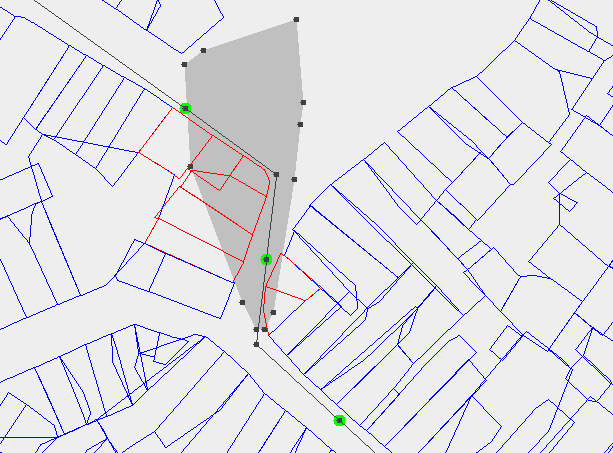
\includegraphics[width=0.48\textwidth]{img/pre3}
    }
    \hfil
     \subfloat{
        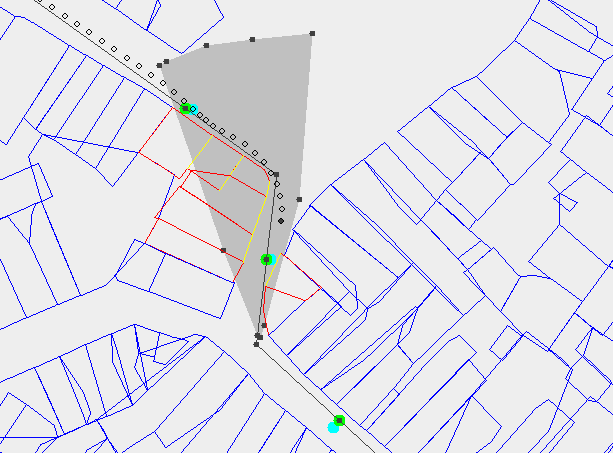
\includegraphics[width=0.48\textwidth]{img/pre4}
     }
    \caption{The left image shows the result after the genetic algorithm has executed. The obstacles in red have been selected to be modeled in the MILP problem. The dark grey shape is the convex allowed region generated by the genetic algortihm. Note how it does not overlap with any of the blue obstacles. The right image shows the final result. The trail of circles show the path of the vehicle up to the current time step, which is represented by the filled circles. The red and yellow colors depict the same information as in figure \ref{fig:obs}}\label{fig:pre-3-4}
\end{figure*}
These corner events are in turn grown outwards to cover the approach and departure from the corner. How much depends on the maximum acceleration of the vehicle. As a rule of thumb: If the vehicle can come to a complete stop from its maximum speed before the corner, it can also successfully navigate that corner. When corners appear in quick succession, their expanded regions may overlap. In that case, the middle between those corners is chosen. Long, straight sections are also divided into smaller path segments.\\
One of the main goals of segmenting the path is to reduce the amount of obstacles. This means that every segment has a set of obstacles associated with it, being the obstacles that need to be modeled for the solver. Not only the obstacle that ``causes'' the corner is important, but obstacles which are nearby are important as well. Obstacles on the outside of the corner also may play a role in how the vehicle approaches the corner. To find all potentially relevant obstacles, the convex hull of the (Theta*) path segment is calculated and scaled up slightly. Every obstacle which overlaps with this shape is considered an active obstacle for that path segment. The convex hull step ensures that all obstacles on the inside of the corner are included, while scaling it up will cover any restricting obstacle on the outside of the corner.
\subsection{Generating the active region for each segment}
Even though the most important obstacles are taken care of, all other obstacles also need to be represented. To do this, a convex polygon is grown around the path. This polygon may intersect with the active obstacles (since they will be represented separately), but may not intersect any other obstacle. The polygon is grown using a genetic algorithm. It uses a single mutator which nudges the vertices of the polygon while ensuring it stays convex and does not intersect itself or any non-active obstacle. The genetic algorithm is just one way to generate the convex polygon which represents the active region. Deits and Tedrake \cite{Deits2015} have demonstrated how another algorithm can solve the same problem.

